\section{Introduction}

Quantum channels, fundamental in the study of quantum information theory,
describe how quantum states evolve under various types of noise and interaction.
These channels serve as models for real-world scenarios where quantum systems
are exposed to external environments, resulting in state transformations that
are often non-ideal. Quantum channels are central to understanding and developing
quantum communication, computation, and cryptography, as they capture the
limitations and potential of transferring quantum information through noisy or
imperfect media.

In quantum information theory, channels are typically categorized based on their
capacities to transmit information. Just as in classical information theory, where
the Shannon capacity limits the rate at which information can be reliably transmitted,
quantum channels are analyzed through various capacity measures, each capturing
different facets of information transfer. The primary capacities of interest include
\textbf{quantum capacity}, \textbf{classical capacity}, and \textbf{private capacity},
each reflecting the channel's ability to transmit quantum information, classical
information, or private (secure) information, respectively. These capacities vary
depending on the nature and severity of the noise introduced by the channel, making
it essential to understand the characteristics and limitations of each type.

One of the distinctive aspects of quantum channels is that their capacities are not
always additive, a property that contrasts with classical channels. The superadditivity
phenomenon, where multiple channel uses jointly yield a higher capacity than the sum of
individual capacities, adds a layer of complexity to the analysis. For example,
entanglement-assisted strategies can enhance both classical and quantum transmission rates,
exploiting the channel's underlying quantum mechanics to achieve greater efficiency. This
superadditivity highlights the advantage of leveraging quantum properties like entanglement
and coherence for information transmission.

Our term paper explores the nature of quantum channels, and delves into the mathematical
frameworks used to quantify their capacities. We discuss the fundamental concepts underlying
quantum channel capacities, analyze the theoretical limits of information transmission, and
cement theses ideas by taking a suitable example.

Before we begin our discussion on channel capacities though, we need to first define some
basic concepts in Quantum Information Theory. Since Quantum Systems work in a fundamentally
different way compared to their classical counterparts, we must define new quantities and
constructs to take these into account.

\subsection{Trace}
It is helpful for us to introduce the \textbf{Trace} of a square operator. It is defined as:
\begin{equation*}
    Tr[A] \equiv \displaystyle\sum_{i} \langle i | A | i \rangle
\end{equation*}
where $A$ is an operator in the Hilbert space $\mathcal{H}$ and $\{|i\rangle\}$ is a complete
orthonormal basis in $\mathcal{H}$.
We note the following properties about the Trace:
\begin{itemize}
    \item Trace is Linear: $Tr[aA + bB] = aTr[A] + bTr[B]$ where $a$ and $b$ are scalars
    \item Trace is independent of the choice of the basis, as long as it is complete and orthonormal
    \item Trace is Cyclic: $Tr[ABC] = Tr[CAB]$
\end{itemize} 

\subsection{States}

In quantum mechanics, the state of a system encapsulates all the information needed to describe
it and predict the outcomes of measurements. For a simple, isolated quantum system, the state
is typically represented as a \textbf{state vector} (or \textbf{ket}) \( |\psi\rangle \) in a
complex Hilbert space \( \mathcal{H} \). This vector describes a \textbf{pure state}, where the
system is in a specific, well-defined quantum state. Mathematically, pure states satisfy
\( \langle \psi | \psi \rangle = 1 \), indicating that the vector is normalized. For example,
in a two-level quantum system (qubit), a general pure state is represented as
\( |\psi\rangle = \alpha |0\rangle + \beta |1\rangle \), where \( \alpha \) and \( \beta \) are
complex coefficients satisfying \( |\alpha|^2 + |\beta|^2 = 1 \).

It is important to note that the trace of the square of a pure state is 1, or
$Tr[| \psi \rangle^2] = 1$.

However, in many real-world scenarios, systems are not isolated and can exist in \textbf{mixed states},
where they are probabilistically distributed over multiple possible states. Mixed states are described
by \textbf{density operators}, which generalize the concept of quantum states to incorporate
probabilistic mixtures and interactions with external environments. Trace of squares of mixed states is
not necessarily 1. $\rho = 0.5 |0 \rangle \langle 0| + 0.5 |1 \rangle \langle 1|$ is an example of such
a mixed state.

In quantum information theory, we define a quantity called \textbf{purity} to judge if a state is pure
or not:

\begin{definition}[Purity]
    The purity of a state $P[\rho]$ is defined as:
    \begin{equation*}
        P[\rho] = Tr[\rho^\dagger\rho] = Tr[\rho^2]
    \end{equation*}
    $P[\rho] = 1$ if $\rho$ is pure and $P[\rho] < 1$ if $\rho$ is NOT pure.
\end{definition}

\subsection{Density Operators}

As described above, the \textbf{density operator} (or \textbf{density matrix})
is a mathematical tool that describes the state of a quantum system. Unlike a pure state, which
represents a system with complete certainty about its state vector, the density operator allows
for the representation of mixed states, where a system may exist in a probabilistic mixture of
several possible states. This flexibility makes density operators essential for describing
real-world quantum systems, particularly when dealing with noise, entanglement, and decoherence
effects in quantum channels. The density operator for a system encodes all observable properties
of the system.

Mathematically, a density operator $\rho$ corresponding to the ensemble $\mathcal{E} \equiv
\{p_X(x), |\psi\rangle \}_{x \in \mathcal{X}}$ is defined as:
\begin{equation*}
    \rho \equiv \displaystyle\sum_{x \in \mathcal{X} } p_X(x) |\psi \rangle \langle \psi|
\end{equation*}
This definition of density operators can also be interpreted as the state of the system. One
more way of understanding the density operator is to think of it as the expected state:
\begin{equation*}
    \rho = \mathbb{E}_X \{ |\psi \rangle \langle \psi| \}
\end{equation*}
The definition gives us a wide picture of the Density operator. As a consequence of the above,
the Density operator has certain properties that it always satisfies. These are summarized here
as follows:
\begin{itemize}
    \item Density operator has unit trace: $Tr[\rho] = 1$
    \item Density operator is Hermitian: $\rho^\dagger = \rho$
    \item Density operators are positive semi-definite, meaning $\langle \varphi  | \rho | \varphi \rangle \geq 0
    \forall \varphi$ which may be written as $\rho >= 0$
\end{itemize}
It is worth mentioning that every ensemble has a unique density operator, but the opposite
is not necessarily true, and the same density operator could correspond to multiple ensembles.

\subsection{Environment and Reference Systems}

In studying quantum systems, we often introduce reference systems and environments to clarify
how entanglement, decoherence, and information transfer occur. A reference system $R$ is often
used as an ancillary(additional) system that helps track information about another system $A$.
Reference systems are useful for defining quantities like coherent information and entanglement.
By examining how the information in $A$ relates to the reference $R$, we gain insights into the
entanglement properties and capacities of quantum channels or systems.

In realistic scenarios,
no quantum system is completely isolated. An environment $E$ represents everything outside the
system of interest, which may interact with it and cause decoherence—the process by which a quantum
system loses its coherence and behaves more classically. When analyzing quantum systems, we model
the system and its environment as a combined entity as mixed states that allow us to study how
noise and information loss occur in quantum channels.

A reference system is often modelled as a \textbf{Product state}:
\begin{definition}[Product State]
    The Tensor Product of a state with another state (often the environment or a reference system).
    \begin{equation*}
        \rho_{AB} = \rho_A \otimes \rho_B
    \end{equation*}
\end{definition}
The product state models all the interactions between the system and the environment. Besides modelling
environment interaction, product states can also model interaction between two systems and give
information about the correlation between them.
\begin{definition}[Bipartite states]
    A state is said to be Bipartite if it is a Tensor Product of two different states.
\end{definition}

This brings us to the related definition of separable states and entanglement:
\begin{definition}[Separable states]
    A bipartite state $\sigma_{AB}$ is said to be Separable if it can be written in the form:
    \begin{equation*}
        \sigma_{AB} = \displaystyle\sum_{x} p_X(x)|\psi_x\rangle\langle\psi_x|_A \otimes |\phi_x\rangle\langle\phi_x|_B
    \end{equation*}
    for some probability distribution $p_X(x)$ and sets $\{| \psi_x \rangle_A\}$ and $\{| \phi_x \rangle_B\}$ of pure states.
\end{definition}

\begin{definition}[Entanglement]
    A state that is not separable is said to be entangled.
\end{definition}

One more tool that is often used in quantum information theory is the Partial Trace. It is defined as follows:

\begin{definition}[Partial Trace]
    Let $X_{AB}$ be a square operator acting on the tensor product Hilbert Space $\mathcal{H}_A\otimes \mathcal{H}_B$
    and let $\{| l \rangle_B\}$ be an orthonormal basis for $\mathcal{H}_B$. Then, the partial trace over $B$ is:
    \begin{equation*}
        Tr_B[X_{AB}] \equiv \displaystyle\sum_{l} (I_A \otimes \langle l |_B) X_{AB} (I_A \otimes | l \rangle_B)
    \end{equation*}
\end{definition}

The partial trace effectively "traces out" one part of the system, leaving us with the "local" density operator to work with.

Now that we have defined the environment, we can go on to describe how a channel process a state. Although
the exact details of a channel will be described below, we are right now interested in describing how
the channel is used to process information.

This usually takes place is 3 steps. As seen in figure \ref{channelimg}, we usually deal with classical
information that needs to be converted to its quantum analogue first. This conversion takes place
through an "encoder", in a process called state preparation. This prepared state can then be evolved
through various quantum channels to get our final result, which is usually quantum information that
needs to be converted to some classical form for analysis through some "decoder". This "decoder" is
more often than not some measurement through some instrument. It is interesting to note that the process
of measurement itself can be modelled as a quantum channel! It is convenient, however, to model
measurements as POVMs (Positive Operator Valuled Measures). We define these as follows:

\begin{definition}[POVM]
    A Positive Operator Valued Measure (POVM) is a set $\{\Lambda_j\}_j$ of operators that satisfy
    non-negativity and completeness:
    \begin{align*}
        \forall j : \Lambda_j \geq 0 \\
        \displaystyle\sum_{j} \Lambda_j = I
    \end{align*}
    and the probability of obtaining outcome $j$ is:
    \begin{equation*}
        \langle \psi | \Lambda_j | \psi \rangle
    \end{equation*}
\end{definition}

\begin{figure}
    \centering
    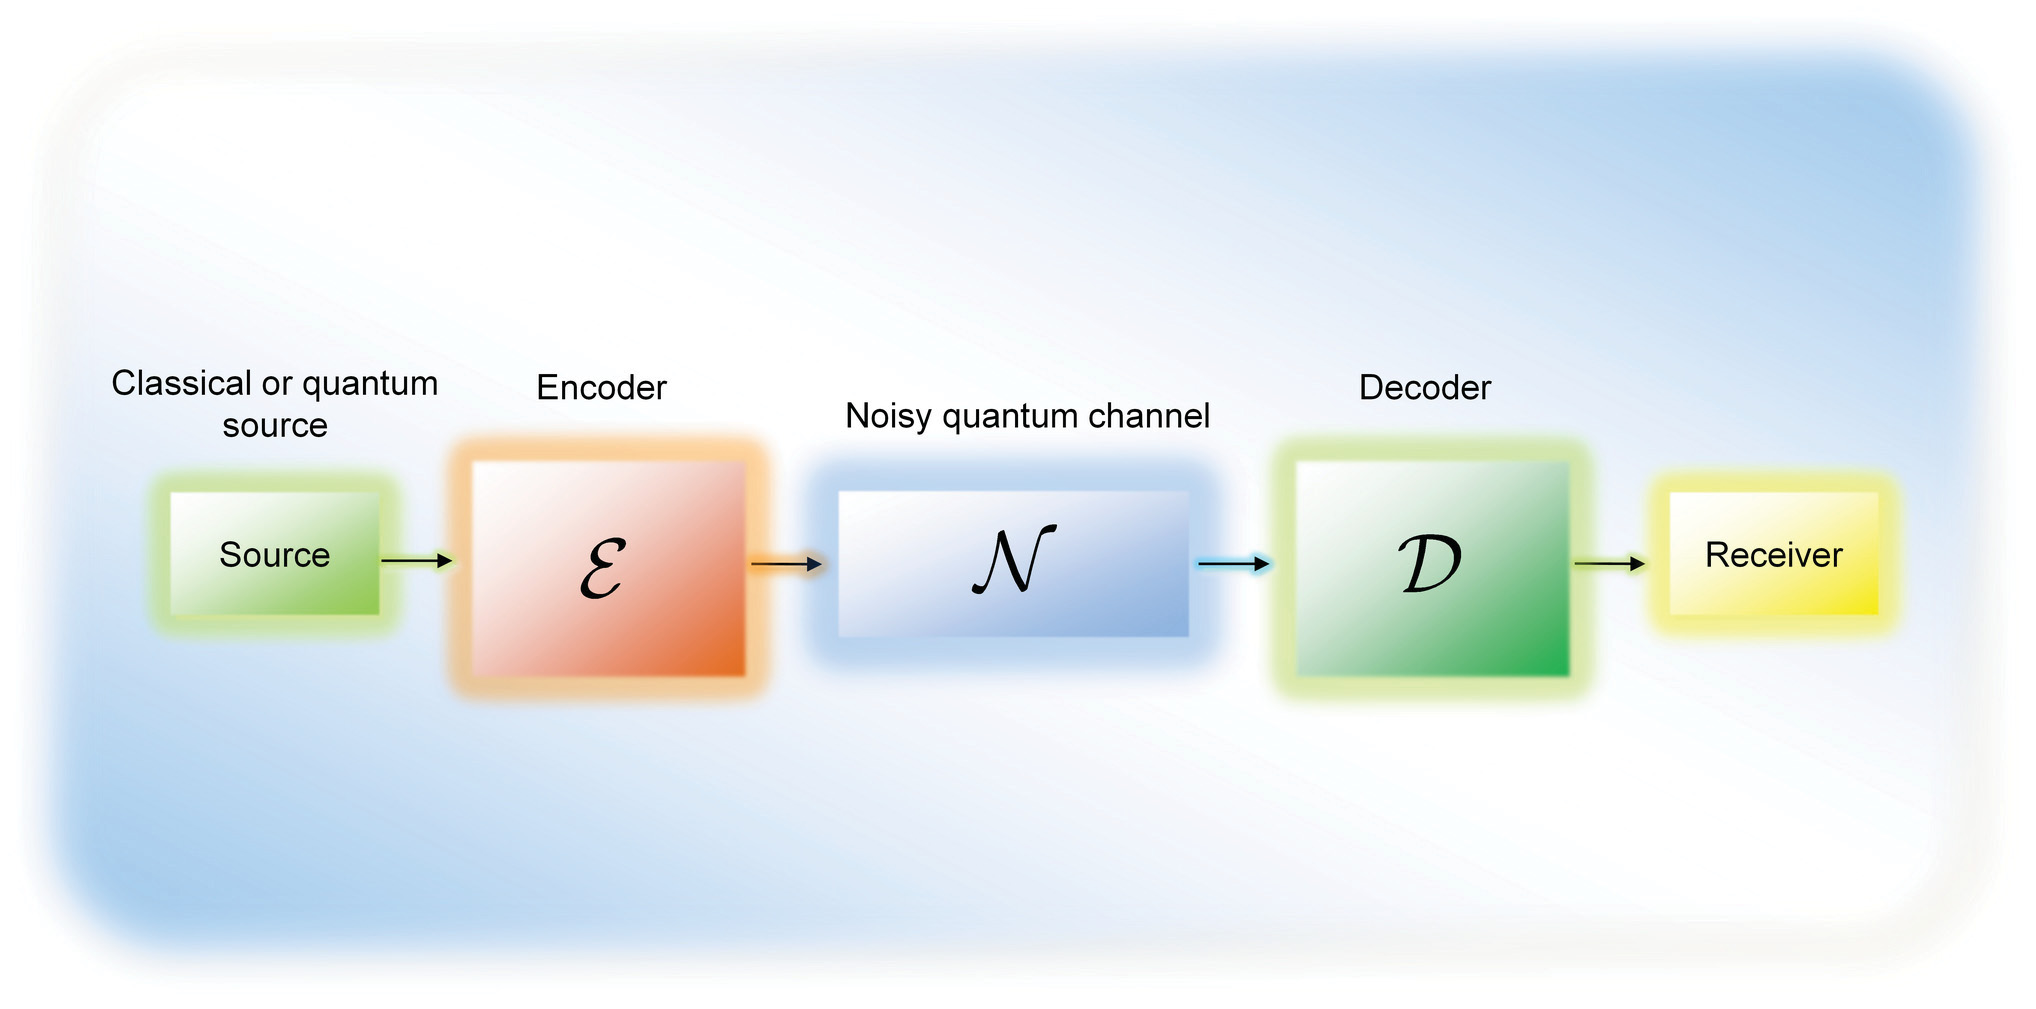
\includegraphics[scale=0.15]{figures/channel1.png}
    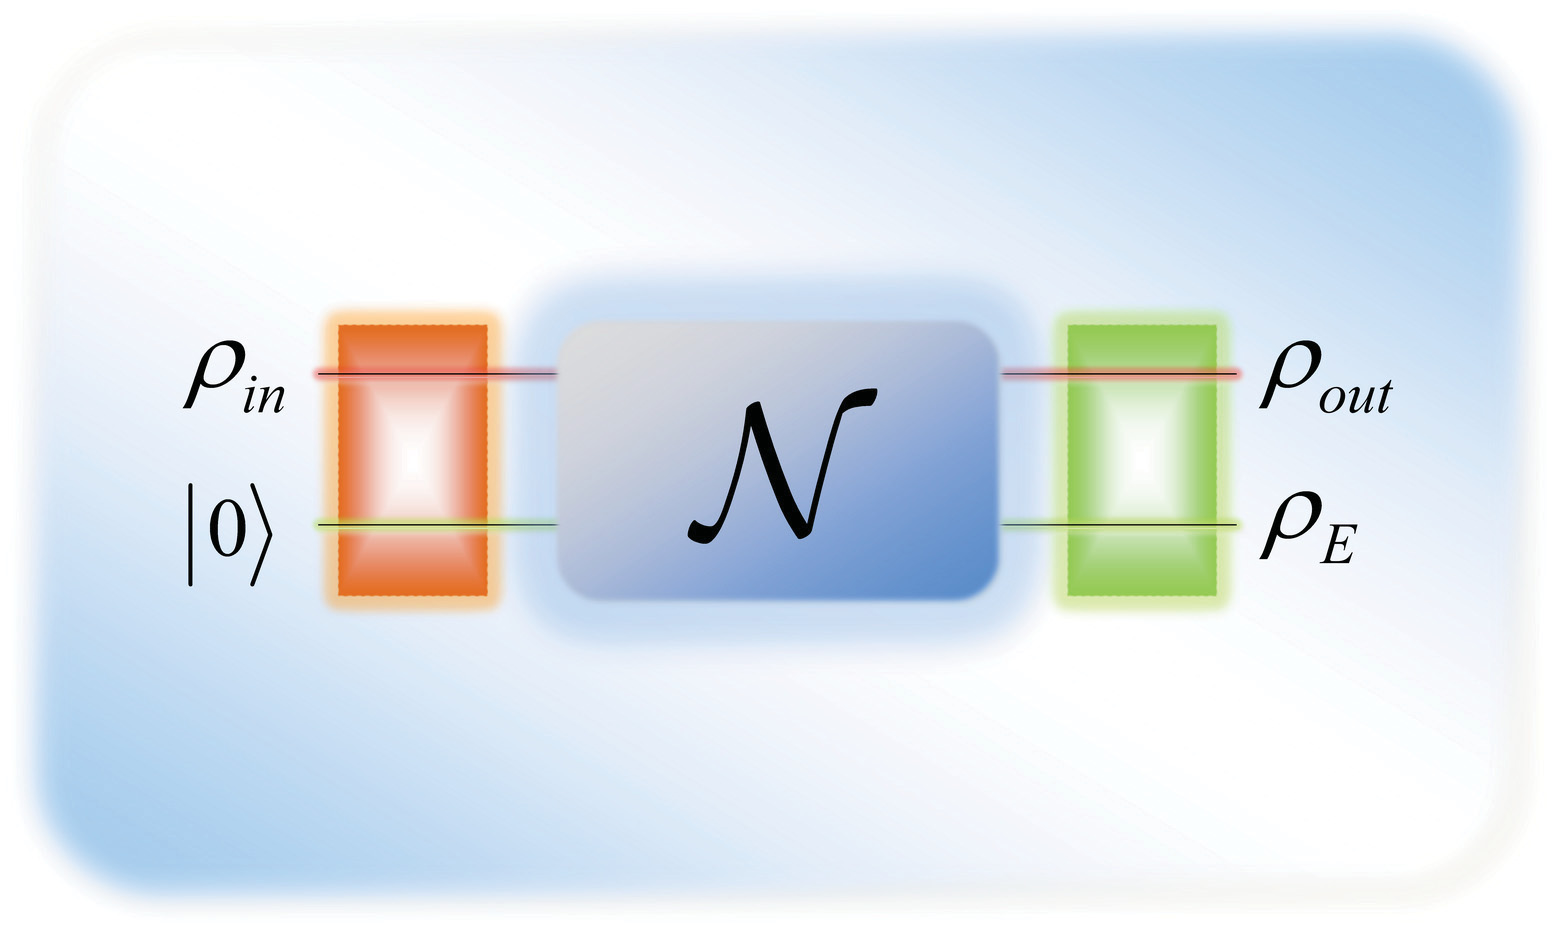
\includegraphics[scale=0.12]{figures/channel2.png}
    \caption{(Top) Illustration of the 3 step process picture of quantum communication, where classical
    information is encoded as quantum information, then evolved through quantum channels, then decoded
    back to classical information - the encoder and decoder can both be modelled as quantum channels
    themselves. (Bottom) Illustration of how a reference system (in this case it is known to be $|0\rangle$)
    may be considered along with the main system when processing through a channel. Images borrowed from \cite{Gyongyosi_2018}}
    \label{channelimg}
\end{figure}

\subsection{Channels as CPTP maps}

Now we have established most things required to begin our major discussion on Quantum Channels. Any
Quantum channel is a model of a physical transformation. Hence, there are certain rules that such a
channel must follow in order to make physical sense.

Let us take $\mathcal{D}_A$ and $\mathcal{D}_B$ to be the set all density operators in Hilbert spaces
$\mathcal{H}_A$ and $\mathcal{H}_B$ respectively. Our channel must be a map from $\mathcal{D}_A$ to
$\mathcal{D}_B$. We use $\mathcal{L}(\mathcal{H})$ to denote the set of all square linear operators on 
$\mathcal{H}$. Let us call our channel $\mathcal{N}$ For the channel to make physical sense, we must
apply 3 restrictions on it:

\begin{description}
    \item[Linearity] {
        It makes sense to have linearity in quantum channels. Although the physical
        basis for this condition is beyond the scope of this short review, if channels were not
        linear, the results of many experiments would not make sense. We may take this as an axiom
        for now.
        
        Hence, a quantum channel must satisfy:
        \begin{equation*}
            \mathcal{N}(\alpha X_A + \beta Y_A) = \alpha \mathcal{N}(X_A) + \beta \mathcal{N}(Y_A)
        \end{equation*}
        }
    \item[Complete Positivity] {
        Since $\mathcal{N}$ maps density operator to density operator, the output of this map must
        be positive semi-definite whenever the input is positive semi-definite as all density operators
        are always positive semi-definite. For this we define positivity:
        \begin{definition}[Positivity]
            A linear map $\mathcal{M} : \mathcal{L}(\mathcal{H}_A) \rightarrow \mathcal{L}(\mathcal{H}_B)$
            is said to be positive if $\mathcal{M}(X_A)$ is positive semi-definite for all positive
            semi-definite $X_A$.
        \end{definition}
        However, this condition must be extended a little bit. Since we are often working with product
        states with reference systems and our channel may apply to only one of the states in the product,
        the above definition may prove to be lacking. To remedy this, we define complete positivity:
        \begin{definition}[Complete Positivity]
            A linear map $\mathcal{M} : \mathcal{L}(\mathcal{H}_A) \rightarrow \mathcal{L}(\mathcal{H}_B)$
            is said to be completely positive if $id_R \otimes \mathcal{M}$ is positive map for a reference
            system $R$ of arbitrary size.
        \end{definition}
        We require our channel map to be completely positive.
    }
    \item[Trace Preserving] {
        Lastly, since (again) our channel maps density operators to density operators, the input and output
        both must have Trace 1. In other words, the trace of the output must be the same as the trace of the
        input. This is defined as:
        \begin{definition}[Trace Preservation]
            A map $\mathcal{N}$ is trace preserving if $Tr[X_A] = Tr[\mathcal{N}(X_A)]$ for all input $X_A \in \mathcal{L}(\mathcal{H}_A)$
        \end{definition}
    }
\end{description}

With the above conditions defined, we may now define a quantum channel:

\begin{definition}[Quantum Channel]
    A quantum channel is a linear, completely positive, trace preserving map, corresponding to a quantum physical evolution.
\end{definition}

\subsection{Choi-Kraus Representation and the Choi operator}

The above definition (CPTP maps) of the quantum channel leads to a certain representation that turns
out to be incredibly useful and insightful. We summarize this representation as the Choi-Kraus theorem:
\begin{theorem}[Choi-Kraus Theorem]
    Any map $\mathcal{N}_{A\rightarrow B}:\mathcal{L}(\mathcal{H}_A) \rightarrow \mathcal{L}(\mathcal{H}_B)$
    (where $\mathcal{L}(\mathcal{H}_A)$ is the space of all Linear operators on $\mathcal{H}_A$) is Linear,
    Completely Positive and Trace Preserving if and only if it has a Choi-Kraus decomposition as follows:
    \begin{equation*}
        \mathcal{N}_{A \rightarrow B}(X_A) = \displaystyle\sum_{l=0}^{d-1} V_l X_A V_l^\dagger
    \end{equation*}
    where $X_A \in \mathcal{L}(\mathcal{H}_A)$, $V_l \in \mathcal{L}(\mathcal{H_A}, \mathcal{H_B})$ 
    $\forall l \in \{0,\dots,d-1\}$ with $d < dim(\mathcal{H}_A)dim(\mathcal{H}_B)$ and
    \begin{equation*}
        \displaystyle\sum_{l=0}^{d-1} V_l^\dagger V_l = I_A
    \end{equation*}
\end{theorem}

Before we provide an outline of the proof, we define Choi operators:

\begin{definition}[Choi Operators]
    Let $\mathcal{H}_R$ and $\mathcal{H}_A$ be isomorphic Hilbert spaces, and let
    $\{| i\rangle_R \}$ and $\{|i\rangle_A \}$ be orthonormal bases for $\mathcal{H}_R$
    and $\mathcal{H}_A$, respectively. Let $\mathcal{H}_B$ be some other Hilbert space,
    and let $\mathcal{N} : \mathcal{L}(\mathcal{H}_A) \rightarrow \mathcal{L}(\mathcal{H}_B)$
    be a linear map (written also as $N_{A\rightarrow B}$). The Choi operator corresponding
    to $N_{A\rightarrow B}$ and the bases $\{| i\rangle_R \}$ and $\{|i\rangle_A \}$ is defined
    as the following operator:
    \begin{equation*}
        (id_R \otimes \mathcal{N}_{A \rightarrow B})(| \Gamma \rangle\langle \Gamma |_{RA})
        = \displaystyle\sum_{i,j = 0}^{d_A-1}| i \rangle\langle j |_R \otimes \mathcal{N}_{A \rightarrow B}(| i \rangle\langle j |_A)
    \end{equation*}
    where $d_A \equiv dim(\mathcal{H}_A)$ and $| \Gamma \rangle_{RA}$ is the unnormalized maximally entangled vector:
    \begin{equation*}
        | \Gamma \rangle_{RA} \equiv \displaystyle\sum_{i=0}^{d_A - 1} | i \rangle_R \otimes | i \rangle_A
    \end{equation*}
\end{definition}

The Choi operator is a profound and very useful tool. The very first thing that we may state
(without proof) is that the positive semi-definiteness of the Choi operator implies the 
complete positivity of the channel map that it corresponds to, and vice versa. This is not
the only information about the channel that the Choi operator carries though. It encodes in
itself the entire behavior of the channel. It is in essence a "finger print" of the channel.

The proof of the Choi-Kraus theorem is very long and beyond the scope of this very short review,
but it uses the Choi operator and various tricks to decompose the channel.

% \renewcommand{\pageauthor}{Yash Seri}

% \subsection{POVM Measurements}
% A \textbf{Positive Operator-Valued Measure (POVM)} is a quantum measurement described by positive semi-definite operators on a Hilbert space. POVMs generalize projection-valued measures (PVMs), allowing for a broader class of quantum measurements. 

% In analogy, while a PVM describes pure state measurements, a POVM is to a \emph{mixed state}, often arising from subsystems of larger quantum systems or effects of noisy environments. POVMs are extensively used in quantum information theory.

% \subsection{Definition}
% Let \( \mathcal{H} \) denote a Hilbert space and \( (X, M) \) a measurable space. A POVM is a function \( F \) defined on \( M \) whose values are positive bounded self-adjoint operators on \( \mathcal{H} \), satisfying:
% \[
% F(X) = I_{\mathcal{H}}, \quad \langle \psi | F(E) | \psi \rangle \geq 0,
% \]
% where \( \langle \psi | F(E) | \psi \rangle \) gives the probability of event \( E \) for state \( |\psi\rangle \). 

% In finite dimensions, a POVM is a set of positive semi-definite Hermitian matrices \( \{F_i\} \) satisfying:
% \[
% \sum_i F_i = I,
% \]
% where \( I \) is the identity matrix.

% \subsection{Properties}
% 1. \textbf{Probability Measure:} For a quantum state \( \rho \), the probability of measurement outcome \( i \) is:
%    \[
%    \text{Prob}(i) = \text{Tr}(\rho F_i).
%    \]
%    If \( \rho \) is pure (\( \rho = |\psi\rangle\langle\psi| \)), this reduces to:
%    \[
%    \text{Prob}(i) = \langle \psi | F_i | \psi \rangle.
%    \]

% 2. \textbf{Comparison with PVMs:} 
%    - In PVMs, measurement operators \( \{P_i\} \) are orthogonal projectors (\( P_iP_j = \delta_{ij}P_i \)).
%    - POVMs relax this restriction, enabling non-orthogonal measurement operators and greater flexibility.

% \subsection{Applications}
% POVMs are widely used in quantum information and communication:
% \begin{itemize}
%     \item \textbf{Quantum State Discrimination:} Optimal strategies for distinguishing non-orthogonal quantum states.
%     \item \textbf{Quantum Cryptography:} Analyze eavesdropping and maximize information extraction.
%     \item \textbf{Quantum Communication:} Determine classical information capacity of quantum channels.
% \end{itemize}

% POVMs generalize quantum measurements, extending beyond projective measurements, and play a crucial role in understanding and utilizing quantum systems.
